% Conference draft: is an iPhone enough as a ground robot's only sensor head and computer?
% Source: thesis Chapter 6 (thesis/chapters/ch6_phone_platform.tex, PRs #18-#20) and
%   Ch5 sec:auto-state-validation (VIO vs OptiTrack table).
% Data: motion-capture sessions Oct 26-27, 2026 (/mnt/project-files/velocity-experiment/);
%   sensor-timing runs Oct 27, 2026 (/mnt/project-files/sensor-timing/summary.csv).
% Every number here appears in one of those sources. \todo{} marks experiments that
% have a protocol and no data yet. Do not fill them by estimate.
\documentclass[conference]{IEEEtran}
\IEEEoverridecommandlockouts

\usepackage{cite}
\usepackage{amsmath,amssymb}
\usepackage{graphicx}
\usepackage{booktabs}
\usepackage{tabularx}
\usepackage{array}
\usepackage{xcolor}
\usepackage{tikz}
\usetikzlibrary{positioning,arrows.meta,decorations.pathreplacing,calc}
\usepackage[hidelinks]{hyperref}

\newcommand{\todo}[1]{\textcolor{red}{[TODO: #1]}}
\newcommand{\tsens}{t_{\text{sensor}}}
\newcommand{\tos}{t_{\text{os}}}
\newcommand{\tqueue}{t_{\text{queue}}}
\newcommand{\tdone}{t_{\text{done}}}

\begin{document}

\title{Is a Phone Enough? Measuring an iPhone as a\\Ground Robot's Only Sensor Head and Computer}

\author{\IEEEauthorblockN{Yojan Gautam}
\IEEEauthorblockA{\todo{affiliation, city, country}\\
\todo{email}}
}

\maketitle

\begin{abstract}
Consumer phones carry cameras, a LiDAR scanner, an IMU, GNSS, a neural accelerator and a battery, which makes them an attractive single board for cheap ground robots.
Earlier phone robots show that the idea works, but none reports whether the phone's own estimates and sensor timing meet the numbers a control loop needs, with every subsystem running at once on a moving vehicle.
We run Terra, a skid-steer rover whose only sensor head and computer is an iPhone with LiDAR, and contribute three things.
First, we turn the rover's control, mapping, detection and guidance stack into nine measurable requirements on the phone.
Second, we compare ARKit visual--inertial odometry (VIO) with OptiTrack motion capture over 17 straight runs.
VIO speed noise, bias, delay and heading meet their requirements, but its speed scale reads 0.912 of truth on average (s.d.\ 0.065, 16 runs, one further run at 0.60).
Third, we introduce a per-hop timing probe that attributes every stale control tick to iOS or to the app.
iOS delivered IMU samples at 99--100~Hz with a 99th-percentile delay of at most 2.3~ms in every run, and all 233 stale ticks in a 336~s run came from an unoptimised Debug build of the app's own depth-to-map step; the Release build had none.
We close with the requirements still open: depth, GNSS and 90-minute endurance.
\end{abstract}

\begin{IEEEkeywords}
smartphone robotics, visual--inertial odometry, sensor timing, low-cost mobile robots, field robotics
\end{IEEEkeywords}

% =====================================================================
\section{Introduction}
\label{sec:intro}

A fleet of cheap ground robots covers more ground than one expensive platform, provided each robot is cheap to build, lose and replace.
The dedicated computer and sensor suite are a large part of what makes a robot expensive to field: each needs power and thermal design, a machine image and its own bring-up.
A current phone already holds most of that suite in one sealed, mass-produced package, and software reaches it as an app install.
This paper asks whether that package is good enough to be the robot's \emph{only} sensor head and computer.

Phones have driven robots before~\cite{oros2013smartphone,fong2013smartspheres,muller2021openbot}.
What those works do not report is whether the phone's own pose estimate and sensor timing meet the specific numbers a closed control loop needs, measured on the vehicle, with mapping, detection and video running on the same chip.
Phone VIO, LiDAR, IMU and GNSS have each been benchmarked, but one at a time, hand-held or static, on an otherwise idle phone (Section~\ref{sec:related}).

We study this question on Terra, a skid-steer rover whose sensing, state estimation, mapping, object detection, planning and speed control all run on an iPhone (Fig.~\ref{fig:pipeline}).
Our contributions are:
\begin{enumerate}
\item \textbf{A requirements framework.} Nine requirements R1--R9 on the phone, each derived from the part of the robot that consumes the sensor, with a threshold that a measurement can pass or fail (Section~\ref{sec:req}).
\item \textbf{VIO against motion capture on a ground robot without wheel encoders.} Seventeen straight runs scored against R1--R4 (Section~\ref{sec:vio}).
\item \textbf{A per-hop sensor timing method} that stamps each sample from sensor to control core and attributes every stale control tick to iOS or to the app. Applied to iOS under full robot load, it shows that the IMU stalls we saw in the field came from a Debug build, not from iOS (Section~\ref{sec:timing}).
\end{enumerate}
Section~\ref{sec:verdict} scores the phone against all nine requirements and lists the experiments that remain.

% =====================================================================
\section{Related Work}
\label{sec:related}

\textbf{Phones as robot computers.}
Oros and Krichmar built a teaching robot around an Android phone for about \$350 excluding the phone~\cite{oros2013smartphone}.
NASA's Smart SPHERES added a smartphone to free-flyers aboard the International Space Station~\cite{fong2013smartspheres}.
OpenBot, the closest predecessor to Terra, drives a \$50 body with an Android phone and runs person following and learned navigation, with its detector at 4 to 33 frames per second depending on the phone~\cite{muller2021openbot}.
None of these reports the accuracy of the phone's pose estimate on the robot or the timing of its sensors, and none uses an iPhone, ARKit or LiDAR.

\textbf{VIO on phones.}
ADVIO compared ARCore, ARKit and Tango with academic VIO on hand-held sequences~\cite{cortes2018advio}, following benchmarks on flying-robot hardware~\cite{delmerico2018benchmark}.
Feigl et al.\ found scale errors of up to 14.4~cm per metre for phone and headset VIO on a factory floor~\cite{feigl2020localization}.
Kim et al.\ found ARKit the most accurate of four commercial systems against OptiTrack, but with the phone hand-held or on a car seat, and did not quantify scale~\cite{kim2022benchmark}.
Wu et al.\ proved that VIO on a ground vehicle moving in straight lines or arcs gains unobservable directions, scale among them, and restored them with wheel encoders~\cite{wu2017vinswheels}.
Terra drives straight lines and arcs and has no encoders.

\textbf{Phone depth, IMU and GNSS.}
iPhone and iPad LiDAR has been characterised on static scenes from a hand-held device~\cite{luetzenburg2021iphone,vogt2021ipad,baruch2021arkitscenes}.
Phone IMUs sample at irregular, device-specific rates~\cite{stisen2015smart} and have been characterised for bias and noise on a stationary phone~\cite{kos2016inertial}; camera--IMU time offsets degrade VIO~\cite{li2014temporal}.
Phone GNSS has median errors of 5--8.5~m static~\cite{zandbergen2011agps} and much larger near buildings~\cite{merry2019smartphone}.
On-device inference is benchmarked on idle phones~\cite{ignatov2019aibenchmark,reddi2022mlperfmobile}, and sustained load drives phones into thermal throttling~\cite{xiao2024llmpocket}.

\textbf{Gap.}
To our knowledge no work reports, for iOS, the delay from IMU sample to app and its worst-case gaps under a concurrent ARKit and LiDAR load, nor ARKit's speed scale on a ground robot against motion capture.

% =====================================================================
\section{Platform}
\label{sec:platform}

\begin{figure*}[t]
\centering
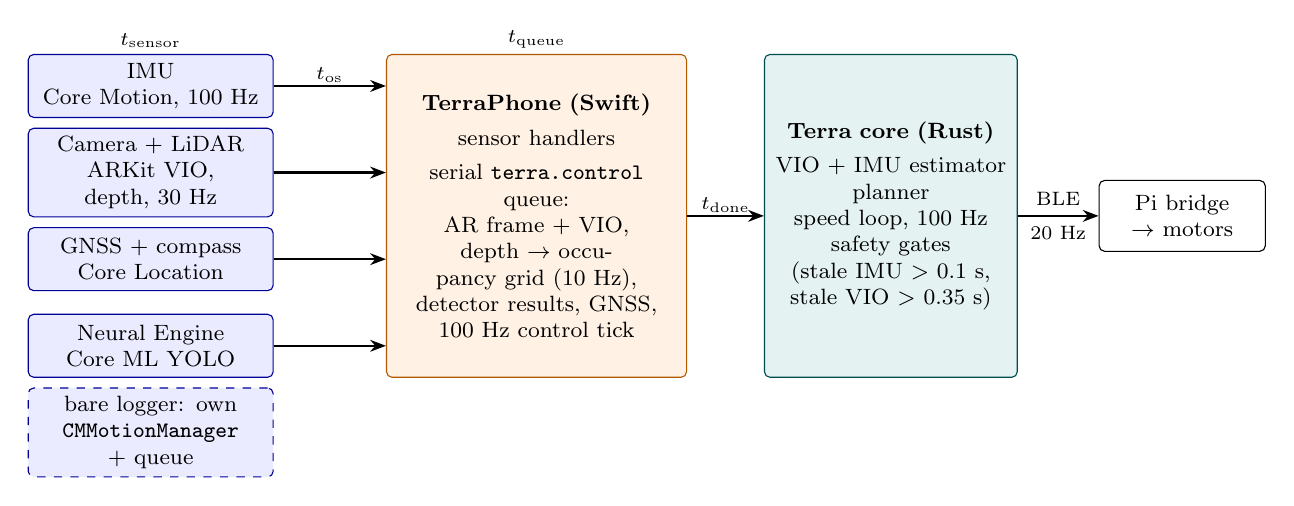
\begin{tikzpicture}[
  box/.style={draw, rounded corners=2pt, align=center, font=\footnotesize, inner sep=3pt},
  ios/.style={box, fill=blue!8, draw=blue!60!black},
  app/.style={box, fill=orange!10, draw=orange!70!black},
  rust/.style={box, fill=teal!10, draw=teal!60!black},
  arr/.style={-{Stealth[length=2mm]}, thick},
  stamp/.style={font=\scriptsize, inner sep=1pt}]
\node[ios, text width=2.9cm, minimum height=0.8cm] (imu) at (0, 2.7) {IMU\\Core Motion, 100~Hz};
\node[ios, text width=2.9cm, minimum height=0.8cm] (cam) at (0, 1.6) {Camera + LiDAR\\ARKit VIO, depth, 30~Hz};
\node[ios, text width=2.9cm, minimum height=0.8cm] (gps) at (0, 0.5) {GNSS + compass\\Core Location};
\node[ios, text width=2.9cm, minimum height=0.8cm] (npu) at (0,-0.6) {Neural Engine\\Core ML YOLO};
\node[app, text width=3.6cm, minimum height=4.1cm] (swift) at (4.9, 1.05) {\textbf{TerraPhone (Swift)}\\[3pt] sensor handlers\\[3pt] serial \texttt{terra.control} queue:\\ AR frame + VIO,\\ depth $\to$ occupancy grid (10~Hz),\\ detector results, GNSS,\\ 100~Hz control tick};
\node[rust, text width=3.0cm, minimum height=4.1cm] (rust) at (9.4, 1.05) {\textbf{Terra core (Rust)}\\[3pt] VIO + IMU estimator\\ planner\\ speed loop, 100~Hz\\ safety gates\\(stale IMU $>$ 0.1~s,\\ stale VIO $>$ 0.35~s)};
\node[box, text width=1.9cm, minimum height=0.9cm] (pi) at (13.1, 1.05) {Pi bridge\\$\to$ motors};
\foreach \s in {imu,cam,gps,npu} \draw[arr] (\s.east) -- (\s.east -| swift.west);
\draw[arr] (swift.east) -- (rust.west);
\draw[arr] (rust.east) -- node[above, font=\scriptsize]{BLE} node[below, font=\scriptsize]{20~Hz} (pi.west);
\node[stamp, above=1pt] at (imu.north) {$\tsens$};
\node[stamp, above] at ($(imu.east)!0.5!(imu.east -| swift.west)$) {$\tos$};
\node[stamp, above=1pt] at (swift.north) {$\tqueue$};
\node[stamp, above] at ($(swift.east)!0.5!(rust.west)$) {$\tdone$};
\node[ios, dashed, text width=2.9cm, minimum height=0.7cm] (bare) at (0,-1.7) {bare logger: own\\\texttt{CMMotionManager} + queue};
\end{tikzpicture}
\caption{Terra's sensing and control pipeline on the phone. Every sample is stamped when the sensor produced it ($\tsens$), when iOS handed it to the app ($\tos$), when its block started on the serial control queue ($\tqueue$), and when it reached the Rust core ($\tdone$). iOS delivery is $\tos-\tsens$ and queue wait is $\tqueue-\tos$. A separate bare logger (dashed) reads Core Motion on its own queue, giving an iOS-only baseline with none of the app's code in the way.}
\label{fig:pipeline}
\end{figure*}

\textbf{Rover and phone.}
The rover is CrabTrapBot, a skid-steer chassis without wheel encoders.
An iPhone with a LiDAR scanner (hardware identifier iPhone17,2, iPhone~16 Pro Max, iOS~27.0.1) is mounted in landscape at a camera height of 0.23~m.
A Raspberry Pi receives wheel commands over Bluetooth Low Energy at 20~Hz and drives the motors; it holds no autonomy and stops the motors if commands stop arriving.
\todo{chassis dimensions, mass, motor and battery spec, and bill of materials with and without the phone.}

\textbf{Software.}
TerraPhone, a Swift app, gathers sensor data, builds a 0.1~m occupancy grid from LiDAR depth, runs a YOLO bucket detector on the Neural Engine and streams video to the operator station.
The Rust core runs the state estimator, planner, safety gates and a 100~Hz speed loop.
The estimator takes the latest ARKit VIO pose and velocity and replays the IMU samples retained since, giving forward speed $\hat v$ and gyro yaw rate $\hat\omega$.
It withholds the estimate, and the controller stops, if VIO reports lost tracking, if the newest IMU sample is older than 0.1~s, or if VIO is older than 0.35~s.
Most phone-side work shares one serial dispatch queue, \texttt{terra.control} (Fig.~\ref{fig:pipeline}): a long block there delays every IMU sample behind it.
The Rust core is always compiled with optimisation; the Swift app is not, in a Debug build.

% =====================================================================
\section{Requirements}
\label{sec:req}

``Good enough'' is testable only against numbers.
Table~\ref{tab:req} derives one requirement for each phone capability from the component of Terra that consumes it.
Where a threshold is a constant in Terra, the table gives its source; where we propose it, the table says so.

\begin{table}[t]
\centering
\caption{Requirements on the phone. ``Proposed'' marks thresholds set in this paper; the rest are constants of the robot.}
\label{tab:req}
\footnotesize
\setlength{\tabcolsep}{3pt}
\begin{tabularx}{\columnwidth}{@{}l >{\raggedright\arraybackslash}p{1.25cm} >{\raggedright\arraybackslash}X >{\raggedright\arraybackslash}p{1.6cm}@{}}
\toprule
ID & Capability & Requirement & Source \\
\midrule
R1 & VIO speed scale & Steady speed within 0.97--1.03 of truth; bias at rest $\le$ 0.01~m/s & Speed-loop accuracy \\
R2 & VIO speed noise & $\le$ 0.02~m/s in the control band & Speed loop \\
R3 & VIO delay & Below the loop's delay margin, 382~ms at the tested gains & Speed-loop stability \\
R4 & Heading & Error $< 30^\circ$ to admit an outdoor mission & Heading gate \\
R5 & IMU delivery & Newest IMU sample younger than 0.1~s at every control tick & Estimator stale gate \\
R6 & Depth & 0.15~m obstacles seen at $\ge$ 3~m; range error $<$ one 0.1~m cell; no false obstacles on bare floor & Map resolution; range proposed \\
R7 & Detection & Recall $\ge$ 0.9 within 10~m above the 0.8 confirm threshold & Target confirm rule; recall proposed \\
R8 & GNSS & 95\% horizontal error $\le$ 10~m & Proposed, from R7's range \\
R9 & Endurance & 90~min of full load without the \emph{critical} thermal state, with battery left & Competition match length \\
\bottomrule
\end{tabularx}
\end{table}

This paper measures R1--R5 and reports the protocols for R6--R9, which are pending (Section~\ref{sec:verdict}).
R5 is the one that most directly decides whether a phone can host a control loop at all, and the one the literature says least about.

% =====================================================================
\section{VIO Against Motion Capture}
\label{sec:vio}

\subsection{Method}

The rover was driven in an OptiTrack volume of about $12 \times 8$~m on October 26 and 27, 2026.
OptiTrack (Motive~3, NatNet~4) tracked a rigid body on the chassis at 120~Hz; over a 3~m tape it read within 0.01~m, so we take it as ground truth.
A bridge republished the mocap pose on the robot's message bus, and one laptop program recorded both poses and drove the rover straight at a set speed and distance through teleoperation.
The phone's own telemetry journal was copied off the phone after each session.
For each run we compare the steady part of the phone's forward speed, after the speed-up and before the stop, with OptiTrack's (Fig.~\ref{fig:vio-example}).
The mocap rigid body sits 0.17~m from the phone's reference point along the forward axis, so on straight runs the lever arm adds no forward speed.

\begin{figure}[t]
\centering
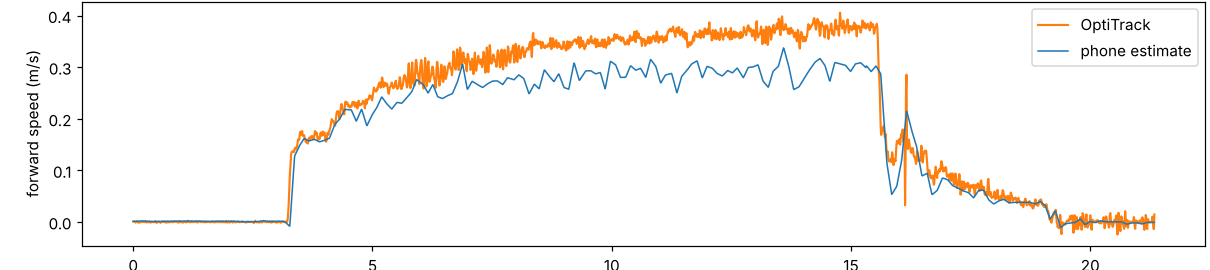
\includegraphics[width=\columnwidth]{figures/vio_example_run.png}
\caption{One straight run at a 0.3~m/s target (session~1, run~2): forward speed from OptiTrack (orange) and from the phone's estimate (blue) against time in seconds. The speed loop holds the phone's estimate near 0.3~m/s while the rover's true speed settles near 0.37~m/s; the steady ratio for this run is 0.81. The phone trace is sparser because the journal recorded it at about 8~Hz.}
\label{fig:vio-example}
\end{figure}

\subsection{Results}

Seventeen straight runs at 0.2--0.4~m/s were usable (Fig.~\ref{fig:vio-ratios}).
Table~\ref{tab:vio} scores them against R1--R4.

\begin{figure}[t]
\centering
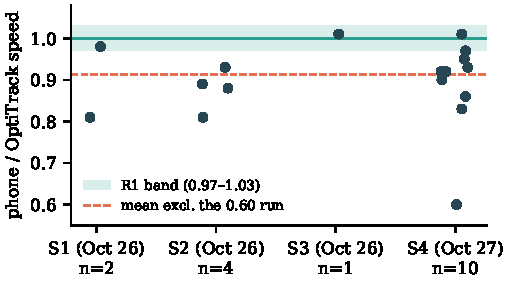
\includegraphics[width=\columnwidth]{figures/vio_scale_ratios.pdf}
\caption{Steady forward speed, phone VIO divided by OptiTrack, for each of the 17 straight runs, by session. Only 4 of the 17 runs fall in the R1 band.}
\label{fig:vio-ratios}
\end{figure}

\begin{table}[t]
\centering
\caption{VIO against OptiTrack, scored against R1--R4.}
\label{tab:vio}
\footnotesize
\setlength{\tabcolsep}{3pt}
\begin{tabularx}{\columnwidth}{@{}l l >{\raggedright\arraybackslash}X l@{}}
\toprule
Req. & Threshold & Measured & Verdict \\
\midrule
R1 scale & 0.97--1.03 & Mean 0.912, s.d.\ 0.065 (16 runs); one run 0.60; all 17: mean 0.894, median 0.92 & Fail \\
R1 bias & $\le$ 0.01~m/s & 0.0009~m/s, s.d.\ 0.003~m/s at rest & Pass \\
R2 noise & $\le$ 0.02~m/s & 0.007~m/s in band, 0.012~m/s above & Pass \\
R3 delay & $<$ 382~ms & About 50--70~ms relative to the gyro & Pass \\
R4 heading & $< 30^\circ$ & Within 0.1$^\circ$ of OptiTrack over a 475$^\circ$ arc & Pass \\
\bottomrule
\end{tabularx}
\end{table}

ARKit gives the speed loop a quiet, unbiased and fast signal with an accurate heading, but its speed scale is about 9\% short and varies from run to run.
Because the loop regulates the phone's estimate, the rover drives faster than commanded by the same factor (Fig.~\ref{fig:vio-example}).
Two further observations bound the cause.
When the rover was carried by hand over 4.42~m (OptiTrack), the phone read 4.06~m, a ratio of 0.92, so the wheels and drive vibration are not the cause.
On one arc, the VIO position jumped by 2.75~m, which a speed loop that differentiates position would see as a spike.
The R3 delay is coarse because the journal sampled the estimate at about 8~Hz.

Two explanations remain.
The first is the room: OptiTrack's infrared strobes may disturb the LiDAR, and the floor is plain.
The second is the motion: Wu et al.\ predict weak scale observability for exactly this straight-line ground motion~\cite{wu2017vinswheels}.
If the room is the cause, the ratio should return to 1 elsewhere; if the motion is, it should stay below 1 in any room and recover only with more varied motion.

\subsection{Pending: scale away from the mocap room (E1b)}
Ground truth is a tape: marks 10.00~m apart, the stop position marked by hand.
Factors are place (mocap room with strobes on, strobes off, textured hallway, plain hallway, outdoor turf), motion (straight, straight with a 1~m side-step weave) and speed (0.3~m/s everywhere; 0.1 and 0.5~m/s in the textured hallway).
With the measured spread of 0.065, 11 runs per cell detect a 0.08 difference between places with 80\% power at $\alpha = 0.05$; detecting 0.05 needs 27.
If one place-independent ratio fits within $\pm$3\%, a fixed scale correction passes R1; otherwise scale needs an independent reference such as GNSS speed outdoors.
\todo{Run E1b (120 runs); add a two-way ANOVA table of ratio on place and motion, and replace this subsection with results.}
\todo{Run E1c: yaw rate in arcs and turns against OptiTrack at 100~Hz logging, after the landscape-mount gyro fix.}

% =====================================================================
\section{Sensor Timing Under Load}
\label{sec:timing}

\subsection{Motivation}

During the mocap sessions and earlier test drives the rover held repeatedly with a stale-IMU fault: at some control tick the newest IMU sample was older than 0.1~s.
A phone's sensor timing is set by the operating system, which the app cannot see into.
The question for R5 is therefore whether the stale samples come from iOS, so that a phone cannot host the loop, or from the app, so that it can be fixed.

\subsection{Per-hop timing probe}

The probe stamps every IMU, AR, detector, GNSS and heading sample at the four points of Fig.~\ref{fig:pipeline} and writes them, with every control tick and every block that ran on the control queue, to a CSV file on the phone.
The \emph{iOS delivery} delay is $\tos - \tsens$; the \emph{queue wait} is $\tqueue - \tos$.
A bare logger, a second Core Motion manager on its own queue, records what iOS delivers with none of Terra's code in the path.

At each control tick the IMU age is $t_\text{tick} - \tsens$ of the newest sample pushed to the Rust core.
When the age reaches the gate, the analysis looks at the \emph{next} IMU sample after the newest one pushed, and assigns the stale tick exactly one cause (Fig.~\ref{fig:attrib}):
\texttt{ios\_sensor\_gap} if that sample had not yet been taken at the tick;
\texttt{ios\_delivery} if it had been taken but iOS had not yet delivered it;
\texttt{terra\_queue} if iOS had delivered it and it was waiting on the control queue, in which case the block running on the queue is named as the blocker.

\begin{figure}[t]
\centering
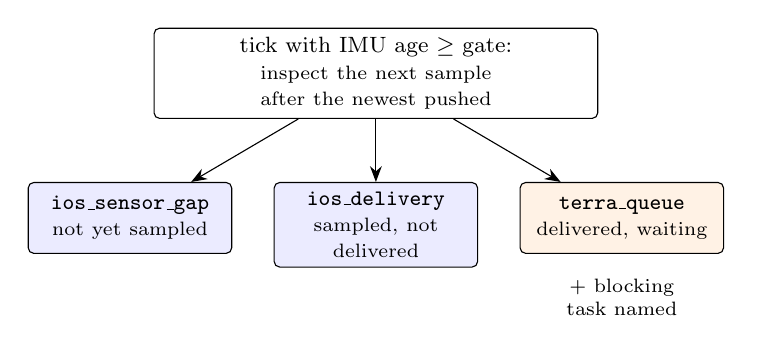
\begin{tikzpicture}[
  q/.style={draw, rounded corners=2pt, align=center, font=\footnotesize, text width=5.4cm, minimum height=8mm},
  leaf/.style={draw, rounded corners=2pt, align=center, font=\footnotesize, text width=2.35cm, minimum height=9mm},
  >={Stealth[length=2mm]}]
  \node[q] (root) {tick with IMU age $\ge$ gate:\\\scriptsize inspect the next sample after the newest pushed};
  \node[leaf, fill=blue!8, below left=8mm and -10mm of root]  (gap) {\texttt{ios\_sensor\_gap}\\\scriptsize not yet sampled};
  \node[leaf, fill=blue!8, below=8mm of root]               (del) {\texttt{ios\_delivery}\\\scriptsize sampled, not delivered};
  \node[leaf, fill=orange!10, below right=8mm and -10mm of root] (que) {\texttt{terra\_queue}\\\scriptsize delivered, waiting};
  \draw[->] (root) -- (gap); \draw[->] (root) -- (del); \draw[->] (root) -- (que);
  \node[below=2mm of que, font=\scriptsize, align=center, text width=2.6cm] {+ blocking task named};
\end{tikzpicture}
\caption{Attribution of a stale control tick. Blue causes are iOS; orange is the app.}
\label{fig:attrib}
\end{figure}

\subsection{Conditions}

All runs used the phone of Section~\ref{sec:platform} on October 27, 2026, with the rover still.
A first short capture gave a pilot for two iOS-only conditions: bare IMU (C0, about 10~s) and IMU with ARKit, LiDAR depth and meshing running (C1, about 7~s).
Four runs then used Terra's full load: tracking on, the detector running (it always runs while tracking, so the \emph{tracking} and \emph{tracking + detector} conditions coincide), and the operator station connected; one Release run added FPV video (C4).
The Debug run lasted 336~s, during which the autonomy level was changed, so we mark it C2$^{*}$.
The Release runs lasted 122, 52 and 38~s, and were recorded after the Debug run with the phone already in the \emph{serious} thermal state.
Debug and Release differ only in the Swift optimiser; iOS and the Rust core are identical.

\subsection{Results}

\begin{table}[t]
\centering
\caption{Sensor timing with Terra's full load, rover still. Stale ticks are control ticks whose newest IMU sample was older than the gate. Detector latency is $\tdone - \tsens$. Thermal state reached \emph{serious} in every run.}
\label{tab:timing}
\footnotesize
\setlength{\tabcolsep}{2.2pt}
\begin{tabular}{@{}l r r r r@{}}
\toprule
 & C2$^{*}$ & C2/C3 & C2/C3 & C4 \\
Build & Debug & Release & Release & Release \\
\midrule
Duration (s) & 336 & 122 & 52 & 38 \\
IMU rate (Hz) & 99.1 & 99.4 & 99.4 & 99.4 \\
iOS delivery p50/p99 (ms) & 0.9/2.1 & 1.0/2.0 & 1.0/2.1 & 1.1/2.3 \\
Queue wait p99 (ms) & 2414 & 8.7 & 14.5 & 20.3 \\
Control queue busy (\%) & 60 & 7 & 10 & 12 \\
Depth-to-map p50/max (ms) & 65.7/114.3 & 9.4/21.9 & 11.8/29.5 & 15.6/28.9 \\
Control tick rate (Hz; 100) & 39.0 & 99.8 & 98.4 & 95.6 \\
IMU age p99/max (ms) & 104/2308 & 14/28 & 19/37 & 24/32 \\
Stale ticks, 0.1~s gate & 233 (1.8\%) & 0 & 0 & 0 \\
Stale ticks, 0.5~s gate & 1 & 0 & 0 & 0 \\
AR frame rate (Hz) & 27.2 & 32.1 & 30.0 & 30.0 \\
Detector rate (Hz) & 4.5 & 4.3 & 4.3 & 4.3 \\
Detector p50/p99 (ms) & 108/172 & 71/80 & 76/91 & 78/97 \\
\bottomrule
\end{tabular}
\end{table}

\textbf{iOS is not the cause.}
In every run iOS delivered IMU samples at 99--100~Hz with a 99th-percentile delay between 2.0 and 2.3~ms (Table~\ref{tab:timing}, Fig.~\ref{fig:ios}), which leaves almost all of the 0.1~s budget to the app.
In the pilot, the bare logger saw p50/p99 delivery of 3.4/4.1~ms with IMU alone (C0) and 1.1/3.0~ms with ARKit, LiDAR and meshing running (C1).
iOS stalled twice in all the data.
It held samples for 1.17~s while an ARKit session started (113 samples held, then delivered in a burst), so a rover must not be allowed to drive until tracking has run for a few seconds.
It also paused the IMU for 2.3~s at 311~s into the Debug run, with the phone in the \emph{serious} thermal state and AR frames gapping by up to 3.8~s at the same time; its cause is unknown.

\begin{figure}[t]
\centering
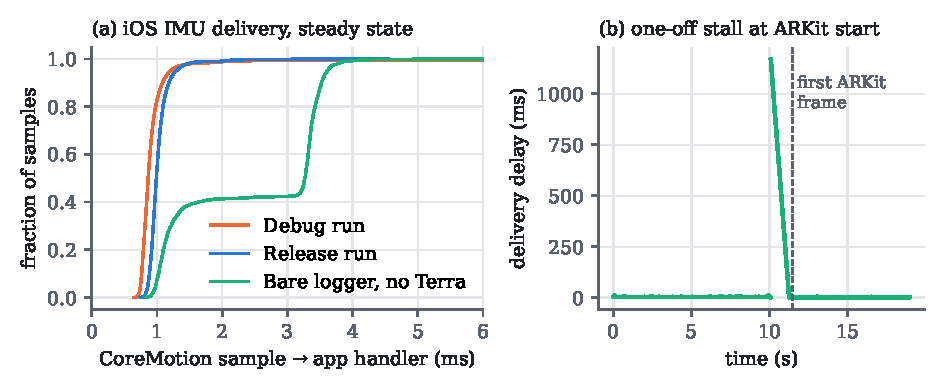
\includegraphics[width=\columnwidth]{figures/phone_timing_ios_delivery.pdf}
\caption{iOS IMU delivery, Core Motion sample to app handler. (a) In steady state, delivery is under about 2~ms in the Debug and Release runs and under 5~ms for the bare logger. (b) The one start-up stall: iOS held samples for 1.17~s while the ARKit session started.}
\label{fig:ios}
\end{figure}

\textbf{The Debug build is the cause.}
All 233 stale ticks of the Debug run were \texttt{terra\_queue}, and in each one the blocker was the Swift depth-to-map step of an AR frame.
That step grew from about 45~ms per frame to over 100~ms during the run (Fig.~\ref{fig:timeline}).
At 10~Hz it kept the control queue 60\% busy, and the 100~Hz control loop averaged 39~Hz.
IMU samples reached the app within about 2~ms and then waited behind the map step.
In Release, the same step took 9--16~ms (p50) and never more than 30~ms, the queue was 7--12\% busy, and the loop ran at 96--100~Hz without a stale tick (Fig.~\ref{fig:dvr}).
The Release runs started with the phone already hot, so heat alone does not explain the Debug slowdown.

\begin{figure}[t]
\centering
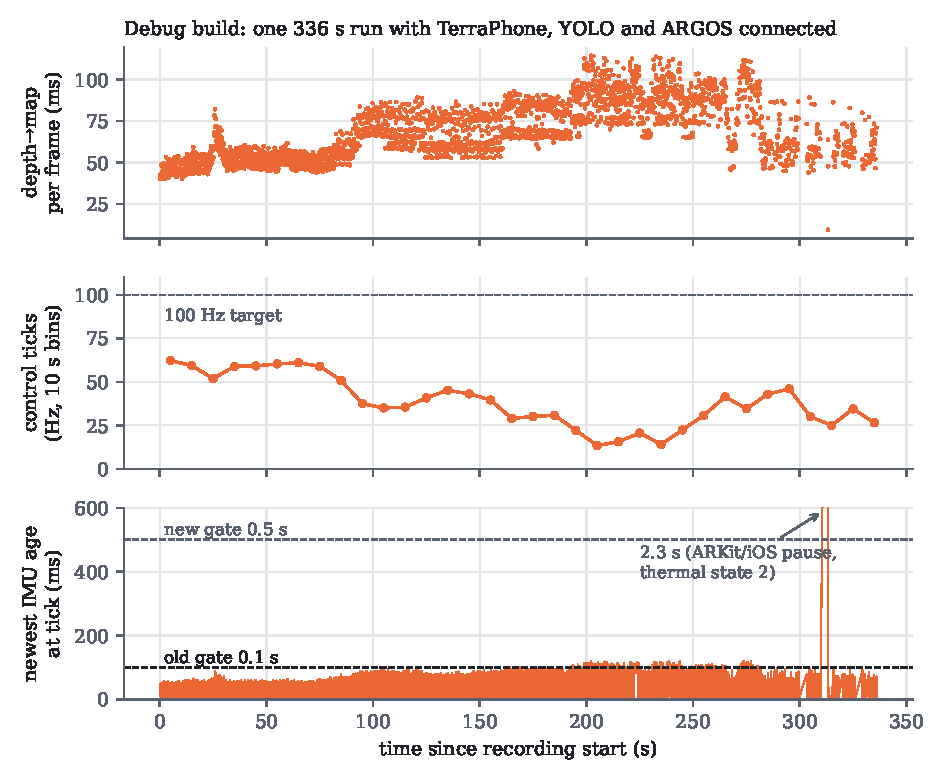
\includegraphics[width=\columnwidth]{figures/phone_timing_debug_timeline.pdf}
\caption{The Debug run (C2$^{*}$, 336~s). Top: time the Swift depth-to-map step held the control queue per frame. Middle: control ticks per second, 10~s bins. Bottom: IMU age at each tick, with the 0.1~s gate and a looser 0.5~s gate.}
\label{fig:timeline}
\end{figure}

\begin{figure}[t]
\centering
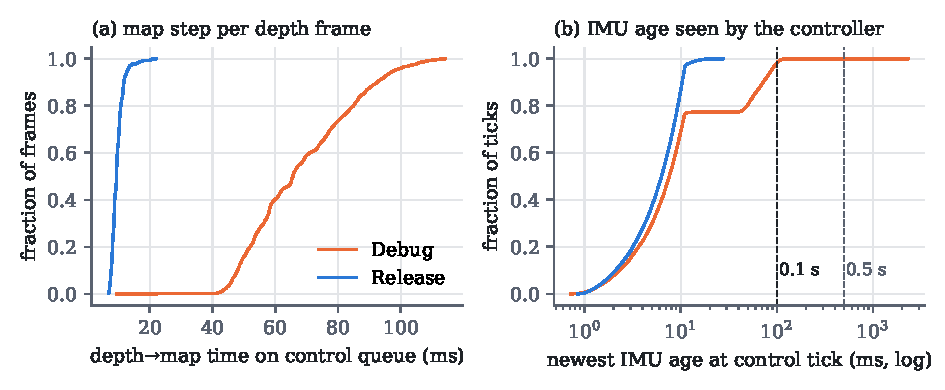
\includegraphics[width=\columnwidth]{figures/phone_timing_debug_vs_release.pdf}
\caption{Debug against Release, empirical CDFs. (a) Depth-to-map time per frame. (b) IMU age at each control tick (log scale) with the 0.1~s and 0.5~s gates.}
\label{fig:dvr}
\end{figure}

Loosening the gate to 0.5~s would have left one stale tick in the Debug run, the 2.3~s iOS pause, instead of 233.
A looser gate hides queue delays rather than removing them, so we take the Release numbers, not the gate, as the evidence for R5.
The broader lesson for phone robotics is methodological: an app's Debug build can turn a sound pipeline into one that looks like the operating system is failing, and only a per-hop probe tells the two apart.

\subsection{Limitations}
The three Release runs total 212~s, none longer than the roughly 150~s the Debug slowdown took to appear; all runs were static; and only one phone model was tested.
\todo{Run a Release run of at least 10 minutes with full load and report whether the late iOS IMU and AR stalls reappear; extend Table~\ref{tab:timing} with it.}
\todo{Run C5: the same probe while driving straight lines at the waypoint and planner autonomy levels.}

% =====================================================================
\section{Verdict and Open Requirements}
\label{sec:verdict}

\begin{table}[t]
\centering
\caption{Is the phone enough? Status of each requirement.}
\label{tab:verdict}
\footnotesize
\setlength{\tabcolsep}{3pt}
\begin{tabularx}{\columnwidth}{@{}l >{\raggedright\arraybackslash}p{1.55cm} >{\raggedright\arraybackslash}X@{}}
\toprule
Req. & Verdict & Basis \\
\midrule
R1 scale & Fail as measured & 0.91 in the mocap room; E1b decides if a fixed correction suffices \\
R2 noise & Pass & Sec.~\ref{sec:vio} \\
R3 delay & Pass & Sec.~\ref{sec:vio} (coarse, 8~Hz journal) \\
R4 heading & Pass (VIO) & Compass and GNSS course pending \\
R5 IMU & Pass in Release; fail in Debug & iOS p99 $\le$ 2.3~ms; Release 0 stale ticks in 212~s; two iOS stalls (1.17~s, 2.3~s); static and short \\
R6 depth & Pending & \todo{E3: targets at 0.5--5~m, four lighting conditions incl.\ mocap strobes and noon sun, parked and driving} \\
R7 detection & Rate measured; accuracy pending & 4.3~Hz, 71/80~ms p50/p99 under full load (Release). \todo{E4: real buckets at 2--12~m, sun and shade} \\
R8 GNSS & Pending & \todo{E5: static CEP50/CEP95 on four surveyed points, 30~m driving runs, compass near motors} \\
R9 endurance & Pending & Serious thermal state after about 4~min in C2$^{*}$ (Debug, still). \todo{E6: 90~min full load, bench and field, battery and thermal logged} \\
\bottomrule
\end{tabularx}
\end{table}

Table~\ref{tab:verdict} collects the status of all nine requirements.
The parts of the phone that the inner control loop depends on most, VIO noise, delay and heading and iOS's IMU delivery, meet their requirements with margin.
The stale-IMU holds that first suggested otherwise came from the app's own unoptimised code on a shared queue and disappeared in Release.
The VIO scale error is real and repeatable in the mocap room; it is small enough that the loop stays stable and the rover stays consistent with its own map, and it matters for absolute distances.
What remains open is the hardest part of the claim: whether all of this holds while driving, outdoors, with every subsystem on for a 90-minute match.
\todo{Fill R6--R9 from experiments E3--E6 and update the abstract and this paragraph.}

% =====================================================================
\section{Conclusion}
\label{sec:conclusion}

We stated what a phone must deliver to be a ground robot's only sensor head and computer as nine testable requirements, and measured the first five on an iPhone driving a skid-steer rover.
ARKit VIO is quiet, unbiased, fast and accurate in heading, but under-reads speed by about 9\% in our mocap room.
iOS delivers IMU samples within about 2~ms under full ARKit, LiDAR, detection and video load; the stalls we first attributed to the phone came from a Debug build, which our per-hop probe exposed.
The probe and analysis scripts are part of the Terra code base.
\todo{State the code and data release (repository URL, licence) once decided.}

\section*{Acknowledgment}
\todo{Advisor, lab, motion-capture facility, funding.}

\bibliographystyle{IEEEtran}
\bibliography{references}

\end{document}
